\documentclass[sigconf]{acmart}
\usepackage{lipsum} 

\settopmatter{printacmref=false} % Removes citation information below abstract
\renewcommand\footnotetextcopyrightpermission[1]{}
\pagestyle{plain} % removes running headers

%%
%% \BibTeX command to typeset BibTeX logo in the docs
\AtBeginDocument{%
  \providecommand\BibTeX{{%
    Bib\TeX}}}

\setcopyright{None}

\settopmatter{printacmref=false}

\begin{document}

\title{Robust Principal Component Analysis on Graphs}

\author{Sofiane Ezzehi}
\affiliation{%
  \institution{École Normale Supérieure Paris-Saclay \\ École des Ponts ParisTech}
  \country{}
}
\email{sofiane.ezzehi@eleves.enpc.fr}

\author{Alexandre Lutt}
\affiliation{%
  \institution{École Normale Supérieure Paris-Saclay \\ École des Ponts ParisTech}
  \country{}
}
\email{alexandre.lutt@eleves.enpc.fr}

\begin{teaserfigure}
  \center
  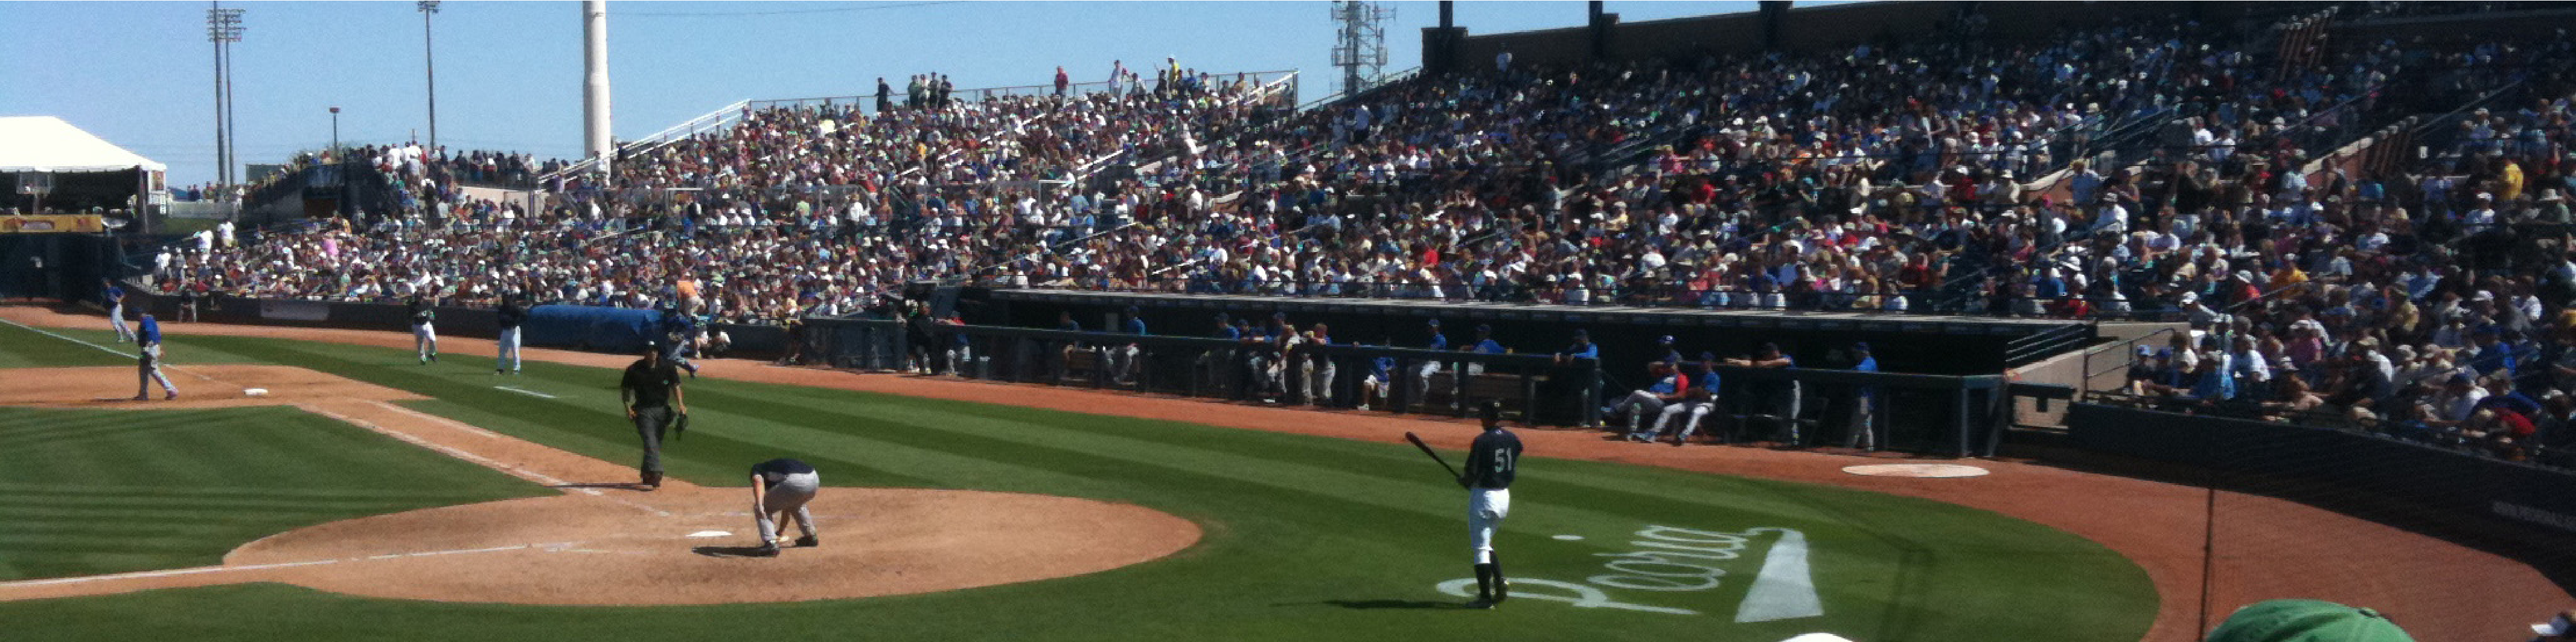
\includegraphics[width=15cm, height=7cm]{sampleteaser}
  \caption{Low-rank reconstruction of corrupted images using the proposed method of~\cite{main_paper}.}
  \Description{Low-rank reconstruction of corrupted images.}
  \label{fig:teaser}
\end{teaserfigure}

\maketitle
\pagestyle{plain}

\section{Abstract}

Principal Component Analysis (PCA) is a very popular method for dimensionality reduction, and is used by thousands accross the world to provide 2D or 3D visualisations and insights about high-dimension data.

However, its main drawback is that it is very sensitive to outliers, and thus cannot be used in many real-world applications.
This issue has been solved by the introduction of a robust variants of PCA, RPCA~\cite{rpca_paper}. However, this algorithm is very slow on large datasets, which makes it impractical for many applications. 
This motivated the introduction of another PCA variant called GLPCA~\cite{glpca_paper} which uses graph Laplacian regularization to improve the robustness of the algorithm while keeping the computational cost low.
Finally, a third variant of PCA similar to the previous ones has been proposed by the authors of~\cite{main_paper} to improve the robustness of the algorithm while keeping the computational cost low.

This project aims to provide a simple and efficient implementation of those main variants of the PCA algorithm, as well as a benchmark of those methods on different tasks (clustering and low-rank recovery for corrupted data on real-life and artificial datsets).


\section{Introduction}




\section{Algorithms}




\section{Experimental setup}




\section{Results}




\section{Limitations}




\section{Conclusion}




%%
%% The next two lines define the bibliography style to be used, and
%% the bibliography file.
\bibliographystyle{ACM-Reference-Format}
\bibliography{bib}

\end{document}
\endinput